\section{Methodology}

\begin{figure}[t] % [h] specifies the placement of the figure
    \centering % Centers the figure
    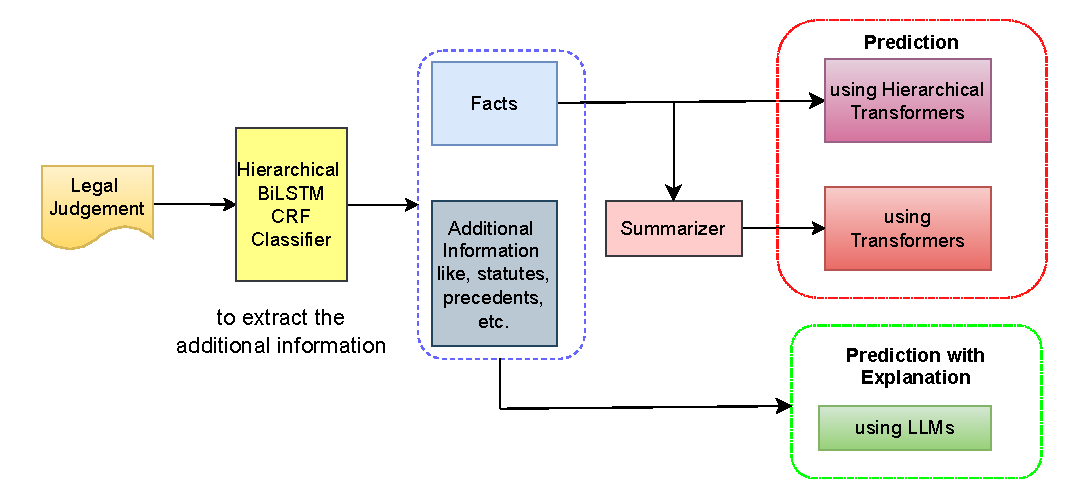
\includegraphics[width=\linewidth]{figures/new_workflow.drawio_cropped.pdf}  
    \caption{Workflow for Legal Judgment Prediction with explanation.}
   \label{fig1}
\end{figure}

%\subsection{Prediction}
\subsection{Extraction of Facts and Additional Information from Judgments}
To extract relevant sentences from legal judgments, we employ a Hierarchical BiLSTM-CRF classifier, focusing on different rhetorical roles as identified by ~\cite{ghosh2019identification}. To create a realistic scenario for our model, we utilize the factual and additional contextual information such as statutes and precedents of the judgments as input for transformer models and LLMs.

\subsection{Transformer and Hierarchical Transformer Models}
The extracted facts undergo summarization using various techniques, including CaseSummarizer ~\cite{polsley2016casesummarizer}, BertSum ~\cite{liu2019fine}, SummaRuNNer ~\cite{nallapati2017summarunner}, and LetSum ~\cite{farzindar2004atefeh}, to ensure they fit within the input constraints of transformer models. Given that models like XLNET-large ~\cite{yang2019xlnet}, BERT ~\cite{devlin2018bert}, and InLegalBERT ~\cite{paul2022pre} can process a maximum input length of 512 tokens, we summarize the facts accordingly. Additionally, we utilize hierarchical transformer models that allow us to input the entire set of facts without the need for summarization. This approach facilitates the handling of comprehensive legal information during the prediction task, which is a binary classification problem.

\subsection{Prediction with Explanation using LLMs}
For the explanation task, we leverage LLMs such as Llama-2 (70b \& 13b) \cite{touvron2023llama} and GPT-3.5 Turbo \cite{brown2020language}, employing a prompting strategy. Given that the combined input and response length for these models is 4096 tokens, we segment the inputs into chunks of 2048 words. This segmentation allows us to generate judgment predictions, as one token corresponds to approximately three-quarters of a word, translating to about 750 words for 1000 tokens\footnote{\href{https://help.openai.com/en/articles/4936856-what-are-tokens-and-how-to-count-them}{what-are-tokens-and-how-to-count-them}}. We then aggregate the outputs from multiple chunks using a majority voting mechanism to determine the final judgment; in the event of a tie, the judgment is considered in favor of the appellant. For inputs shorter than 2048 words, we directly input the entire text into the LLM without requiring majority voting. We explore two prompting techniques:\\
\textbf{Normal Prompting:} The prompt states, ``You are asked to be a judge of a legal case and provide a judgment of the following legal judgment: \verb|<Legal judgment>|."\\
\textbf{Chain-of-Thought Prompting (CoT):} Following the chain-of-thought approach proposed by ~\cite{wei2022chain}, the prompt is modified to include, ``Think Step by Step."

We investigate six variations for each model input including sentences from:\\
\textbf{V1:} Only facts.\\
\textbf{V2:} V1 + statutes, and precedents.\\
\textbf{V3:} V2 + rulings by lower courts.\\
\textbf{V4:} V3 + arguments.\\
\textbf{V1+CoT:} Similar to V1, but incorporates the CoT prompt, ``Think Step by Step."\\
\textbf{V4+CoT:} Similar to V4, but includes the CoT.

Variations V1 and V2 simulate realistic scenarios where only essential elements, such as facts, statutes, and precedents, are provided to the LLM. These components mirror how judges typically approach cases by relying on the factual context and legal frameworks. V3 accounts for cases where a lower court has previously ruled on the matter, adding another layer of realism by simulating situations where an appeal is being heard. V4 enhances the prediction process by including arguments from legal counsel, simulating the complexity of real courtroom proceedings.

Prompting strategies engage both Task A (prediction) and Task B (explanation), thereby facilitating a comprehensive approach to judgment prediction and rationale generation.